\begin{sidewaysfigure*}
  \centering
  % \begin{noindent}
  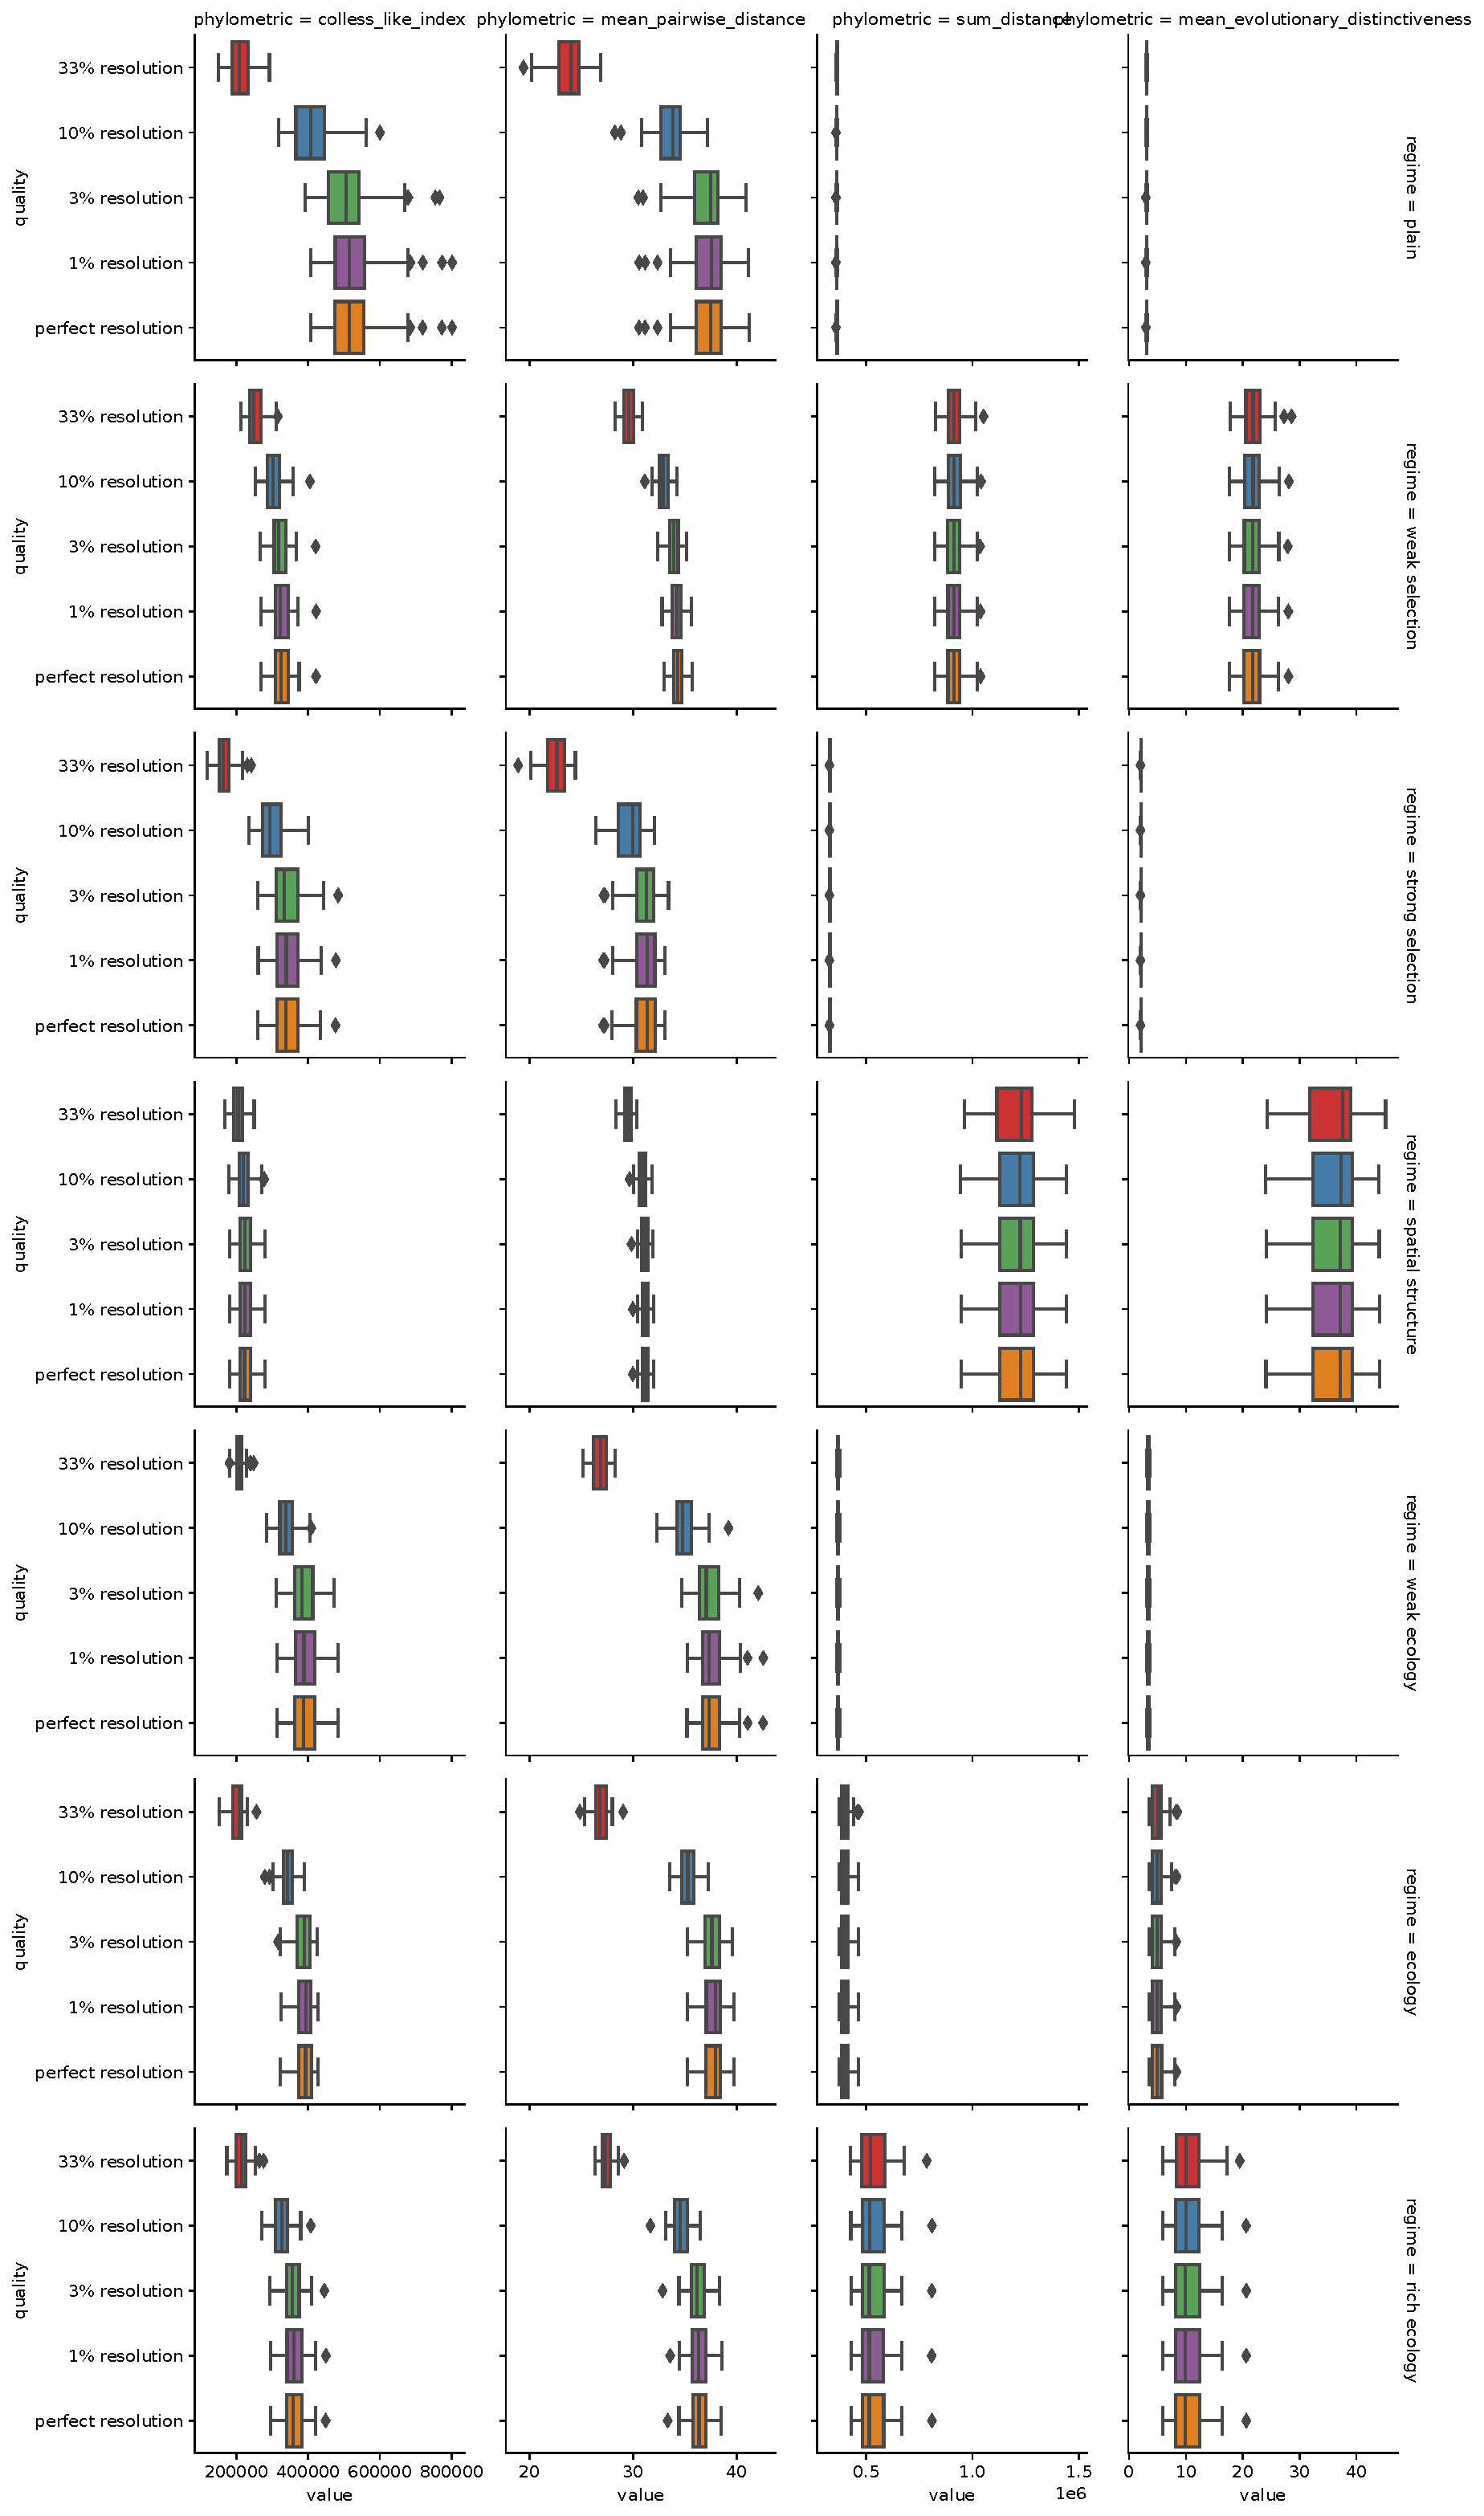
\includegraphics[height=\textwidth,angle=-90]{binder/binder/teeplots/col=phylometric+epoch=7+mut_distn=np.random.standard_normal+row=regime+viz=boxplot+x=value+y=quality+ext=.pdf}
  % \end{noindent}
  \caption{%
    Distributions of phylometrics across surveyed reconstruction fidelities and evolutionary regimes.
    Results are for standard experimental conditions: gaussian mutation distribution at epoch 7 (generation 262,144).
    See Figures \labelcref{fig:reconstructed-tree-phylometrics-epoch0,fig:reconstructed-tree-phylometrics-epoch2,fig:reconstructed-tree-phylometrics-exponential} for results under sensitivity analysis conditions.
    Sample sizes of $n=50$ replicates define each depicted distribution.
  }
  \label{fig:reconstructed-tree-phylometrics}
\end{sidewaysfigure*}
